\section{Testing, Complexity and Results} \label{results}
In order to verify that the solution worked, it was compared to a pre-existing tool which creates trees  similar to this project's, which may be found here: \url{http://mwskirpan.com/FractalTree/}. The difference here is that the number of iterations in this tool starts at 3, whereas this work presents an implementation which starts at 1, hence we must add 2 to our iteration number when testing. The option to change the trunk width is also given by the tool in the link. A comparison may be found in figure \ref{fig:comparison}. The reason why our version looks squashed is because it was output to a square image, and as discussed before, the tree will stretch to the image size, showing that the method is working properly. Multiple angles and heights were tested, giving matching results. Edge cases, such as when the y-values go below 0, were also considered and the program works without any known errors.

\begin{figure}
	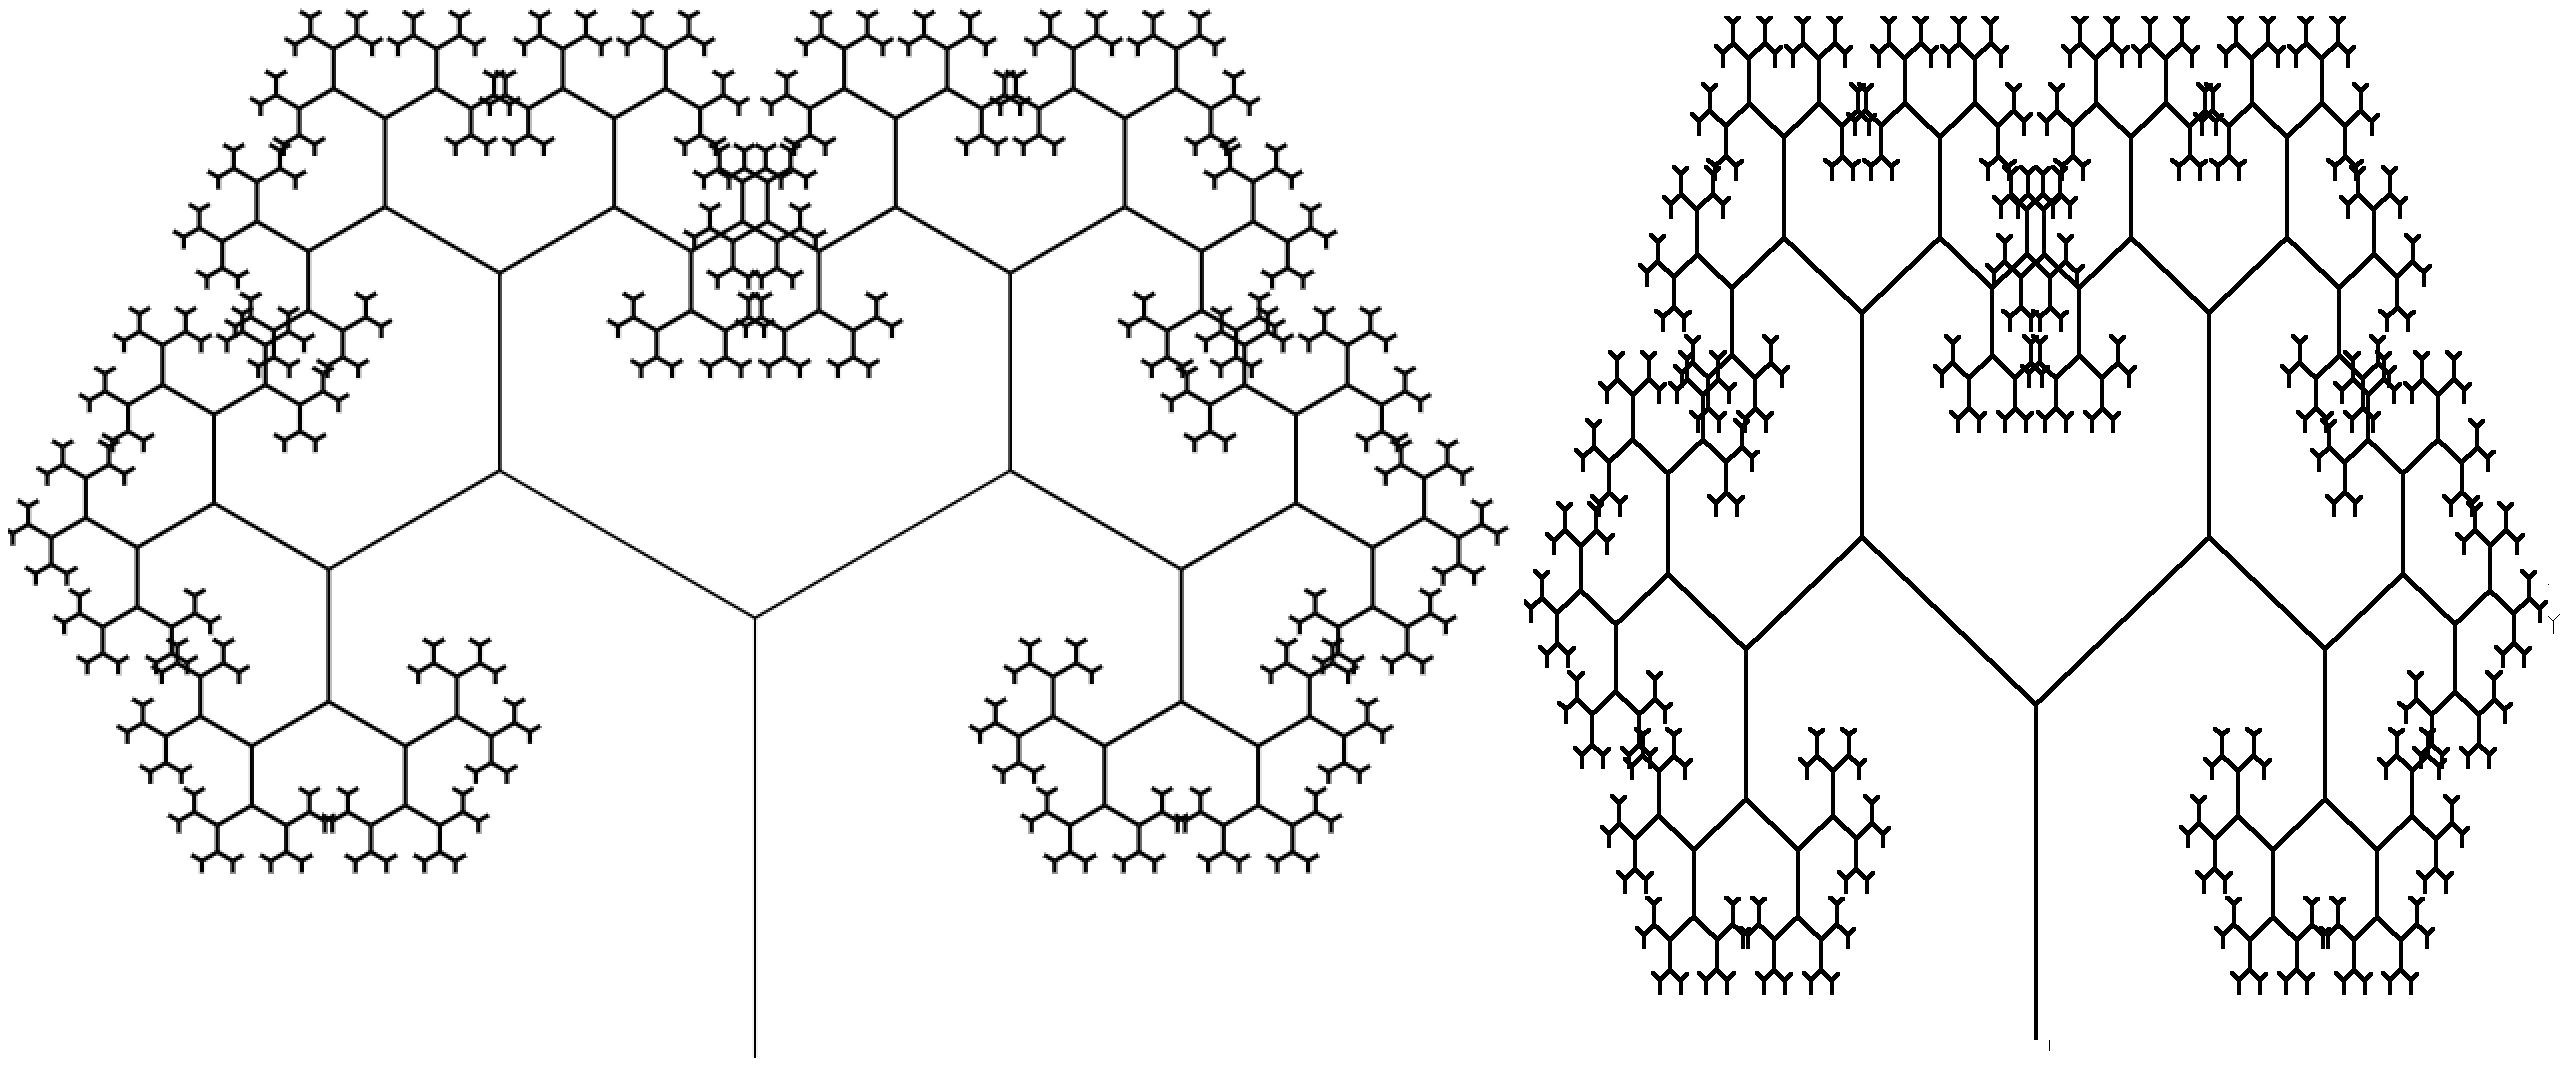
\includegraphics[width=\linewidth]{Images/Comparison.png}
	\centering
	\caption{A comparison of our method (right) and the pre-existing version (left). The parameters are: $m=0.67, n=10, angle=60$}
	\label{fig:comparison}
\end{figure}

Results of timing will be given for 1) the generation of points and 2) Image synthesis, separately. This means that these will be considered as two tasks, as they will scale up differently with different parameters. These comparisons were made on an Intel Core i7-3632QM 2.2GHz with Turbo Boost up to 3.2GHz. First we show results the first task, which in theory scales with O($2^n$). This entails the generation of the sine and cosine maps, the generation of points and the mapping of these points from coordinate to pixel space. The graph showing the time increase for this first part can be seen in figure \ref{fig:iterVStime}. The exact values of the last 4 points are as follows:
\begin{itemize}
	\item 23 iterations : 0.276479s
	\item 24 iterations : 0.57129s
	\item 25 iterations : 1.16521s
	\item 26 iterations : 2.43377s
\end{itemize}
The exact values can differ by a few milliseconds from one run to the next, but it can be clearly seen that as the number of iterations is increased by 1, the time taken becomes approximately twice what it was with 1 less iteration.

\begin{figure}
	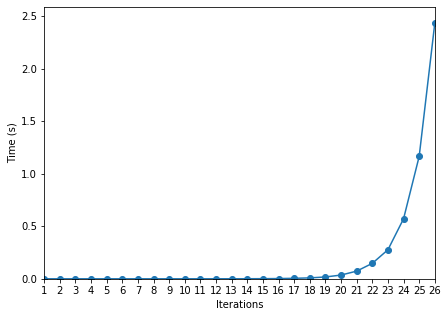
\includegraphics[width=\linewidth]{Images/iterationsVStime.png}
	\centering
	\caption{A graph of the time taken to compute the position of each point in image space against the number of iterations, while all other variables are kept constant, with m=1, theta=90 degrees and image size 1024x1024}
	\label{fig:iterVStime}
\end{figure}

Next, part 2 is examined. 10 runs are performed twice. The first time we only adjust one of the dimensions (the width in this case) of the image (figure \ref{fig:widthVStime}), and the second we adjust both by the same amount, while keeping all other variables constant (figure \ref{fig:dimVStime}).

\begin{figure}
	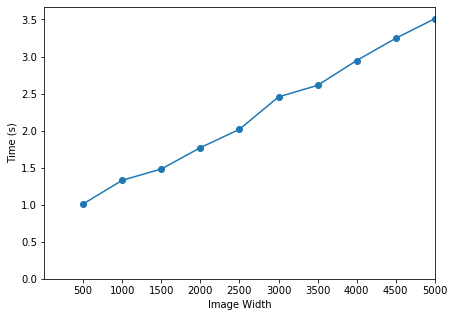
\includegraphics[width=\linewidth]{Images/widthVStime.png}
	\centering
	\caption{A graph of the time taken to draw all the lines in the image against the width of the image, while all other variables are kept constant, with m=1, n=20, theta=90 degrees and an image height of 1024}
	\label{fig:widthVStime}
\end{figure}

From the graph in figure \ref{fig:widthVStime}, it can be seen that changing the width has a linear relationship with the time.

The next graph in figure \ref{fig:dimVStime} shows time taken to draw the lines on the image matrix against the dimensions of the image, where the width and height are equal at each point (so at the first point they are both equal to 500, in the next they are both equal to 1000, and so on). This graph shows that even when both change, the relationship is still linear. From this graph we can infer 2 things. The first is that filling the image matrix, even though this is O(W*H), where W is the width and H is the height, does not affect the performance that much in the scope of our program, as this is a relatively easy task to perform on 'small' ($\ge$5000 pixels) image sizes. Meanwhile, changing the image width or height will incur a change of O(W+H) when drawing the lines.

\begin{figure}
	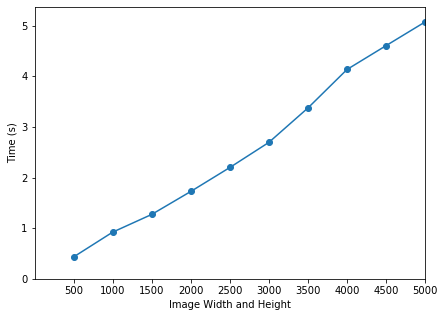
\includegraphics[width=\linewidth]{Images/dimVStime.png}
	\centering
	\caption{A graph of the time taken to draw all the lines in the image against the dimensions of the image, while all other variables are kept constant, with m=1, n=20, theta=90 degrees}
	\label{fig:dimVStime}
\end{figure}

This second part also scales O($2^n$) with the number of iterations since each line needs to be drawn, however, we now also know the complexity with regards to the width and height of the desired output image. The graph for the time taken to draw the lines against the number of iterations can be seen in figure \ref{fig:iterVStimeImage}. So we can say that the total complexity for this second part is O($(W+H)*2^n$).

\begin{figure}
	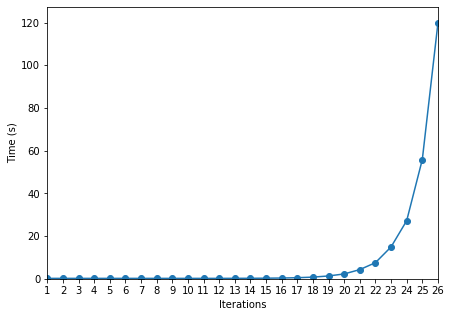
\includegraphics[width=\linewidth]{Images/iterVStimeImage.png}
	\centering
	\caption{A graph of the time taken to draw all the lines in the image against the number of iterations, while all other variables are kept constant, with m=1, n=20, theta=90 degrees and image size 2500x2500}
	\label{fig:iterVStimeImage}
\end{figure}

After doing the parallel implementation, similar results will be presented to determine any performance difference, if any, and why the results came to be.